\documentclass{article}
\usepackage{amsmath}
\usepackage{graphics}
\usepackage{listings}
\title{Implementation of exponential function in C}
\author{Martin Aagaard}
\date{}
\begin{document}
\maketitle 
\begin{abstract}
In this short report an implementation of the exponential function
will be investigated.  
\end{abstract}

\section{The exponential function}
The exponential function is widely known and used and can be defined through the
property that $\frac{d y(x)}{dx} = y$ if $y(x)=e^x$. The exponential function
appears many places e.g. in physics which necessitates an implementation in
computer languages. One way to do this is through the taylor series of the
exponential function, 

\begin{align}
e^x=\sum^{\infty}_{n=0} \frac{x^n}{n!} \label{Taylor_exp} \; . 
\end{align}

\section{Implementation}
From the taylor series it is seen that one can take factor out factors of x and 
n leading to an expression on the following form:
\begin{align}
1+x\cdot(1+\frac{x}{2}\cdot(1+\frac{x}{3}\cdot(...))) \; .
\end{align}
This odd form of writing the series minimizes the number of time a program would
need to multiply and through that minimizing the operation time. 
In C a final implementation could look like:
\begin{lstlisting}[language=C]
double ex(double x){
if(x<0)return 1/ex(-x);
if(x>1./8)return pow(ex(x/2),2);
return 1+x*(1+x/2*(1+x/3*(1+x/4*(1+x/5*(1+x/6*(1+x/7*(1+
x/8*(1+x/9*(1+x/10)))))))));
} . 
\end{lstlisting}
Here the if statements make sure that the value of x is significantly small to
use double precision and not negative since summing alternating values will make
the routine lose precision from subtracting and adding small numbers.
As for significantly small values of x, it is here calculated that for
$10^{-15}$ precision with 10 terms, a value of x smaller than $\frac{1}{8}$ is 
needed. 
This allows us to include fewer terms of the taylor series.

\section{Result}
The implementation is now compared to the exp-function from math.h. The result
is seen in figure~(\ref{fig:exp})
	\begin{figure}
% GNUPLOT: LaTeX picture with Postscript
\begingroup
  \makeatletter
  \providecommand\color[2][]{%
    \GenericError{(gnuplot) \space\space\space\@spaces}{%
      Package color not loaded in conjunction with
      terminal option `colourtext'%
    }{See the gnuplot documentation for explanation.%
    }{Either use 'blacktext' in gnuplot or load the package
      color.sty in LaTeX.}%
    \renewcommand\color[2][]{}%
  }%
  \providecommand\includegraphics[2][]{%
    \GenericError{(gnuplot) \space\space\space\@spaces}{%
      Package graphicx or graphics not loaded%
    }{See the gnuplot documentation for explanation.%
    }{The gnuplot epslatex terminal needs graphicx.sty or graphics.sty.}%
    \renewcommand\includegraphics[2][]{}%
  }%
  \providecommand\rotatebox[2]{#2}%
  \@ifundefined{ifGPcolor}{%
    \newif\ifGPcolor
    \GPcolorfalse
  }{}%
  \@ifundefined{ifGPblacktext}{%
    \newif\ifGPblacktext
    \GPblacktexttrue
  }{}%
  % define a \g@addto@macro without @ in the name:
  \let\gplgaddtomacro\g@addto@macro
  % define empty templates for all commands taking text:
  \gdef\gplbacktext{}%
  \gdef\gplfronttext{}%
  \makeatother
  \ifGPblacktext
    % no textcolor at all
    \def\colorrgb#1{}%
    \def\colorgray#1{}%
  \else
    % gray or color?
    \ifGPcolor
      \def\colorrgb#1{\color[rgb]{#1}}%
      \def\colorgray#1{\color[gray]{#1}}%
      \expandafter\def\csname LTw\endcsname{\color{white}}%
      \expandafter\def\csname LTb\endcsname{\color{black}}%
      \expandafter\def\csname LTa\endcsname{\color{black}}%
      \expandafter\def\csname LT0\endcsname{\color[rgb]{1,0,0}}%
      \expandafter\def\csname LT1\endcsname{\color[rgb]{0,1,0}}%
      \expandafter\def\csname LT2\endcsname{\color[rgb]{0,0,1}}%
      \expandafter\def\csname LT3\endcsname{\color[rgb]{1,0,1}}%
      \expandafter\def\csname LT4\endcsname{\color[rgb]{0,1,1}}%
      \expandafter\def\csname LT5\endcsname{\color[rgb]{1,1,0}}%
      \expandafter\def\csname LT6\endcsname{\color[rgb]{0,0,0}}%
      \expandafter\def\csname LT7\endcsname{\color[rgb]{1,0.3,0}}%
      \expandafter\def\csname LT8\endcsname{\color[rgb]{0.5,0.5,0.5}}%
    \else
      % gray
      \def\colorrgb#1{\color{black}}%
      \def\colorgray#1{\color[gray]{#1}}%
      \expandafter\def\csname LTw\endcsname{\color{white}}%
      \expandafter\def\csname LTb\endcsname{\color{black}}%
      \expandafter\def\csname LTa\endcsname{\color{black}}%
      \expandafter\def\csname LT0\endcsname{\color{black}}%
      \expandafter\def\csname LT1\endcsname{\color{black}}%
      \expandafter\def\csname LT2\endcsname{\color{black}}%
      \expandafter\def\csname LT3\endcsname{\color{black}}%
      \expandafter\def\csname LT4\endcsname{\color{black}}%
      \expandafter\def\csname LT5\endcsname{\color{black}}%
      \expandafter\def\csname LT6\endcsname{\color{black}}%
      \expandafter\def\csname LT7\endcsname{\color{black}}%
      \expandafter\def\csname LT8\endcsname{\color{black}}%
    \fi
  \fi
    \setlength{\unitlength}{0.0500bp}%
    \ifx\gptboxheight\undefined%
      \newlength{\gptboxheight}%
      \newlength{\gptboxwidth}%
      \newsavebox{\gptboxtext}%
    \fi%
    \setlength{\fboxrule}{0.5pt}%
    \setlength{\fboxsep}{1pt}%
\begin{picture}(7200.00,5040.00)%
    \gplgaddtomacro\gplbacktext{%
      \csname LTb\endcsname%%
      \put(814,946){\makebox(0,0)[r]{\strut{}$0$}}%
      \put(814,1430){\makebox(0,0)[r]{\strut{}$20$}}%
      \put(814,1914){\makebox(0,0)[r]{\strut{}$40$}}%
      \put(814,2398){\makebox(0,0)[r]{\strut{}$60$}}%
      \put(814,2883){\makebox(0,0)[r]{\strut{}$80$}}%
      \put(814,3367){\makebox(0,0)[r]{\strut{}$100$}}%
      \put(814,3851){\makebox(0,0)[r]{\strut{}$120$}}%
      \put(814,4335){\makebox(0,0)[r]{\strut{}$140$}}%
      \put(814,4819){\makebox(0,0)[r]{\strut{}$160$}}%
      \put(946,484){\makebox(0,0){\strut{}$-5$}}%
      \put(1532,484){\makebox(0,0){\strut{}$-4$}}%
      \put(2117,484){\makebox(0,0){\strut{}$-3$}}%
      \put(2703,484){\makebox(0,0){\strut{}$-2$}}%
      \put(3289,484){\makebox(0,0){\strut{}$-1$}}%
      \put(3875,484){\makebox(0,0){\strut{}$0$}}%
      \put(4460,484){\makebox(0,0){\strut{}$1$}}%
      \put(5046,484){\makebox(0,0){\strut{}$2$}}%
      \put(5632,484){\makebox(0,0){\strut{}$3$}}%
      \put(6217,484){\makebox(0,0){\strut{}$4$}}%
      \put(6803,484){\makebox(0,0){\strut{}$5$}}%
    }%
    \gplgaddtomacro\gplfronttext{%
      \csname LTb\endcsname%%
      \put(209,2761){\rotatebox{-270}{\makebox(0,0){\strut{}$y$}}}%
      \put(3874,154){\makebox(0,0){\strut{}$x$}}%
      \csname LTb\endcsname%%
      \put(5816,4646){\makebox(0,0)[r]{\strut{}ImplExp}}%
      \csname LTb\endcsname%%
      \put(5816,4426){\makebox(0,0)[r]{\strut{}exp}}%
    }%
    \gplbacktext
    \put(0,0){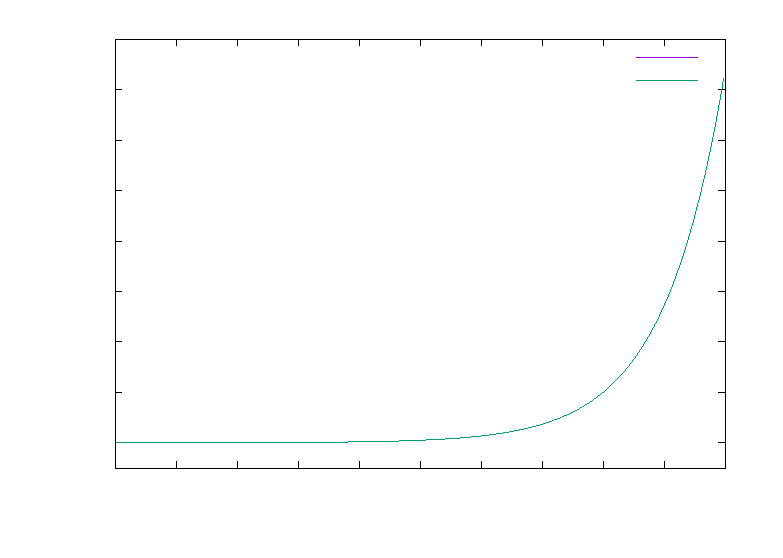
\includegraphics{exp_plot}}%
    \gplfronttext
  \end{picture}%
\endgroup

\caption{Implementated exponential function (Implexp) compared with the math.h 
implemantation(exp) via gnuplot "latex" terminal.}
\label{fig:exp}
	\end{figure} 

\end{document}

